\section{Einleitung}
\label{sec:Einleitung}

Ziel dieses Versuches ist es, die effektive Masse der Leitungselektronen in Galliumarsenid (GaAs) zu bestimmen.
Dafür wird der Faraday-Effekt ausgenutzt und eine Vergleichsmessung zwischen reinem und dotiertem GaAs durchgeführt,
um den Effekt der Leitungselektronen zu isolieren.

\section{Theorie}
\label{sec:Theorie}

Für diesen Versuch wird Galliumarsenid verwendet, es handelt sich dabei um einen Halbleiter.
GaAs kann undotiert oder dotiert vorliegen, von besonderem Interesse für diesen Versuch sind n-dotierte
Varianten, da diese Leitungselektronen aufweisen.
Allgemein besitzen alle Festkörper ein Valenzband sowie ein Leitungsband, dies wird auch als Bandstruktur bezeichnet. Im Valenzband befinden sich
die Elektronen, die für die kovalenten Bindungen zwischen den Atomen zuständig sind.
Das Leitungsband kann nur von Elektronen besetzt werden, wenn diese eine minimal benötige Energie besitzen.
In Halbleitern ist diese Energie etwas höher als die Fermi-Energie der Elektronen, weshalb Elektronen
nur durch Anregung in das Leitungsband wechseln können.
Elektronen im Leitungsband verleihen dem Festkörper eine elektrische Leitfähigkeit, da sie sich
im Gegensatz zu Elektronen im Valenzband nahezu frei bewegen können.
Diesen Leitungselektronen lässt sich
eine effektive Masse zuordnen, welche in diesem Versuch bestimmt werden soll und im nächsten Kapitel
näher erläutert wird.

\subsection{Effektive Masse}

Zum Verständniss der effektiven Masse bietet es sich an, die Bandstruktur eines Halbleiters im k-Raum
zu betrachten. Diese ist in \autoref{fig:Halbleiter} graphisch dargestellt.

\begin{figure} [H]
    \centering
    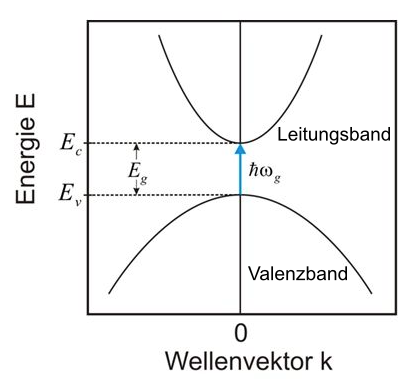
\includegraphics[height=8cm]{content/Halbleiter.png}
    \caption{Bandstruktur eines Halbleiters im k-Raum. \cite{Halbleiter}}
    \label{fig:Halbleiter}
\end{figure}

Hierbei beschreibt $E_{\text{v}}$ die maximale Energie des Valenzbandes und $E_{\text{c}}$ die minimale Energie des Leitungsbandes.
Damit ein Elektron vom Valenzband ins Leitungsband wechseln kann, muss ihm die Energie $E_{\text{g}}=\hbar \omega_{\text{g}}$
zugeführt werden.
Im Bereich um $k=0$ weißt die Bandstruktur einen nahezu parabelförmigen Verlauf auf, weshalb sich eine Taylorentwicklung der unteren Kante des
Leitungsbandes bis zur zweiten Ordnung anbietet:

\begin{equation}
    E(\vec{k})=E\left(0\right)+\frac{1}{2}\sum_{i=1}^3\left(\frac{\partial E^2}{\partial k_i^2}\right)_{k=0}k_i^2+...\,
    \notag
\end{equation}
 
Verglichen mit einem harmonischen Oszillator mit

\begin{equation}
    E=\frac{\hbar k^2}{2m}\,
    \notag
\end{equation}

fällt auf, dass sich der zweite Koeffizient der Taylorentwicklung als effektive Masse $m_i^*$ interpretieren lässt:
    
\begin{equation}
    m_i^*:=\frac{\hbar^2}{\left(\frac{\partial\epsilon^2}{\partial k_i^2}\right)_{k=0}}
    \notag
\end{equation}

Unter der Annahme, dass der Kristall in alle Richtungen nahezu symmetrisch ist, kann eine allgemeine effektive Masse
$m^*$ definiert werden, die sich eignet, um die Dynamik der Leitungselektronen zu beschreiben. Im wesentlichen
lassen sich die Leitungselektronen somit als freie Elektronen beschreiben, deren Wechselwirkung mit dem Kristallgitter
über die veränderte Masse $m^*$ beschrieben wird.

\subsection{Zirkulare Doppelbrechung}
\label{sec:Faraday}

In optisch aktiven Medien kann zirkulare Doppelbrechung auftreten. Diese beschreibt die
Fähigkeit eines Kristalles, die Polarisationsebene eines linear polarisierten Lichtstrahles bei der Transmission zu drehen, das Konzept ist in 
\autoref{fig:rotation} dargestellt.

\begin{figure} [H]
    \centering
    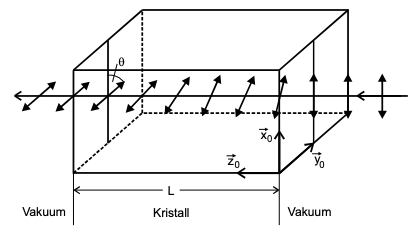
\includegraphics[height=6cm]{content/rotation.png}
    \caption{Zirkulare Polarisation in einem Kristall. \cite{V46Anhang}}
    \label{fig:rotation}
\end{figure}

Die Ursache liegt dabei darin, dass Phasengeschwindigkeiten für links- und rechtszirkular polarisiertes Licht in dem Kristallmedium verschieden sind.
Hierbei kann linear polarisiertes Licht gemäß \autoref{eq:supo} als Überlagerung von links- und rechtszirkular polarisiertes Licht verstanden werden.
\begin{equation}
    E(z)=\frac{1}{2}(E_\text{L}(z)+E_\text{R}(z))
    \label{eq:supo}
\end{equation}
Beim Durchqueren des Mediums findet nun aufgrund der unterschiedlichen Geschwindigkeiten eine Rotation der Polarisationsrichtung statt.
Der Rotationswinkel in Abhängigkeit der Phasengeschwindigkeiten lautet
\begin{equation}
    \theta = \frac{L\omega}{2}(\frac{1}{v_{\text{Ph}_r}}-\frac{1}{v_{\text{Ph}_l}})
    \notag
\end{equation}
beziehungsweise über die Brechungsindices ausgedrückt
\begin{equation}
    \theta = \frac{L\omega}{2}(\frac{1}{n_{\text{r}}}-\frac{1}{n_{\text{l}}}).
    \label{eq:winkel}
\end{equation}
Dabei ist $L$ die Länge des Kristalls und $\omega$ die Kreisfrequenz der elektromagnetischen Welle.
Die unterschiedlichen Phasengeschwindigkeiten kommen aufgrund der Dipolmomente der Atome auf den Gitterplätzen im Kristall sowie
der Wechselwirkung der Bandelektronen mit diesen zustande. Deshalb kann der in \autoref{eq:winkel} berechnete Winkel mithilfe einiger
Umformungen über die Suszeptibilität ausgedrückt werden:
\begin{equation}
    \theta = \frac{L\omega}{2cn}\chi_{xy}
    \label{eq:thetatensor}
\end{equation}

\subsection{Faraday Effekt}

Durch das Anlegen eines Magnetfeldes parallel zur Ausbreitungsrichtung des Lichtes kann in einem optisch inaktiven Medium die selbe Rotation erzeugt werden, dies
wird auch als Faraday Effekt beschrieben. Der physikalische Hintergrund ist hierbei, dass die Leitungselektronen durch das Magnetfeld auf Kreisbahnen
gezwungen werden und Dipolmomente erzeugen.
Die Tensorkomponente $\chi_{xy}$ aus \autoref{eq:thetatensor} ergibt sich nun zu
\begin{equation}
    \chi_{xy} = \frac{N\text{e}^3\omega B}{\epsilon_0\left(\left(-m\omega^2+K\right)^2-\left(\text{e}\omega B\right)^2\right)}
    \label{eq:tensor}
\end{equation}
Dabei beschreibt $K$ die Bindungskonstante der Elektronen an ihre Umgebung.
Das Einsetzen von \autoref{eq:tensor} in \autoref{eq:thetatensor} liefert die Beziehung
\begin{equation}
    \theta=\frac{\text{e}_0^3\omega^2NBL}{2\epsilon_0cm^2\left(\left(-\omega^2+\omega_0^2\right)^2-\left(\omega_{\text{c}}\omega\right)^2\right)n}
    \label{eq:ha}
\end{equation}
wobei $\sqrt{\frac{K}{m}}$ als Resonanzfrequenz $\omega_0$ definiert wurde sowie $\omega_{\text{c}} = \frac{\text{e}B}{m}$ für die Zyklotronfrequenz steht.
Zuletzt wird angenommen, dass die Messfrequenz $\omega$ wesentlich kleiner als $\omega_0$ ist, sowie dass $\omega_0>\omega_{\text{c}}$ gilt. Dann vereinfacht
sich \autoref{eq:ha} zu der Formel
\begin{equation}
    \theta(\lambda)=\frac{\text{e}_0^3}{8\pi^2\epsilon_0c^3}\frac{1}{{m^*}^2}\frac{NBL}{n}\lambda^2\,
    \label{eq:theta}
\end{equation}
welche die Rotation der Polarisationsebene in Abhängigkeit der Wellenlänge angibt.
Sind alle vorkommenden Größen bekannt, also das Magnetfeld $B$, die Ladungsträgerdichte $N$ und die Länge der Probe $L$, kann die effektive Masse
$m^*$ durch Umstellen von \autoref{eq:theta} berechnet werden.
Aus praktischen Gründen wird mit $\theta_\text{frei}$ gerechnet, hier wird der Rotationswinkel $\theta$ auf die Länge der Probe normiert.